\subsection{Co-Simulations and SIL / HIL}

Co-simulations are used to model and analyze complex systems with multiple
interacting components, each of which may have different properties and
behaviors. They involve combining simulation models from different domains, such
as control, power, and thermal management, to create a unified model that
accurately represents the behavior of the overall system.

One of the main advantages of co-simulations over regular simulations is their
ability to capture the interactions between different components of the system.
Regular simulations often make simplifying assumptions that can lead to
inaccurate results. Co-simulations, on the other hand, can account for the
interactions between components and provide a more accurate representation of
the system's behavior. This makes co-simulations particularly useful for
designing and optimizing complex systems like datacenters. The virtual
environment can save time and resources, reduce the risk of failure, and lead to
more efficient and sustainable datacenters \cite{vogt2018}.

Co-simulations can be further enhanced by incorporating the SIL and HIL
methodology. This approach involves integrating real-world components, such as
software and hardware, into the simulation environment to better reflect the
actual system behavior. The integration of real components allows for a more
accurate representation of the system's behavior and can also identify potential
issues that may arise in real-world scenarios \cite{kelemenova2013}.

\subsection{Mosaik}

Mosaik is an open-source co-simulation tool that allows for the integration of
different simulation models from various domains into a unified simulation
environment. Mosaik provides a Python-based framework for developing and
executing co-simulations, enabling the creation of complex simulations with
interacting components. Mosaik supports the development of co-simulation
scenarios by providing an API for defining simulation models, connecting them to
form a simulation network, and specifying simulation scenarios. The tool also
provides various visualization tools and data analysis capabilities to analyze
the results of the simulation. Mosaik allows for the integration of simulation
models from different domains, by providing a library of pre-existing simulation
models that can be used to build custom simulations.

\subsection{Ecovisor}

\begin{figure}
    \centering
    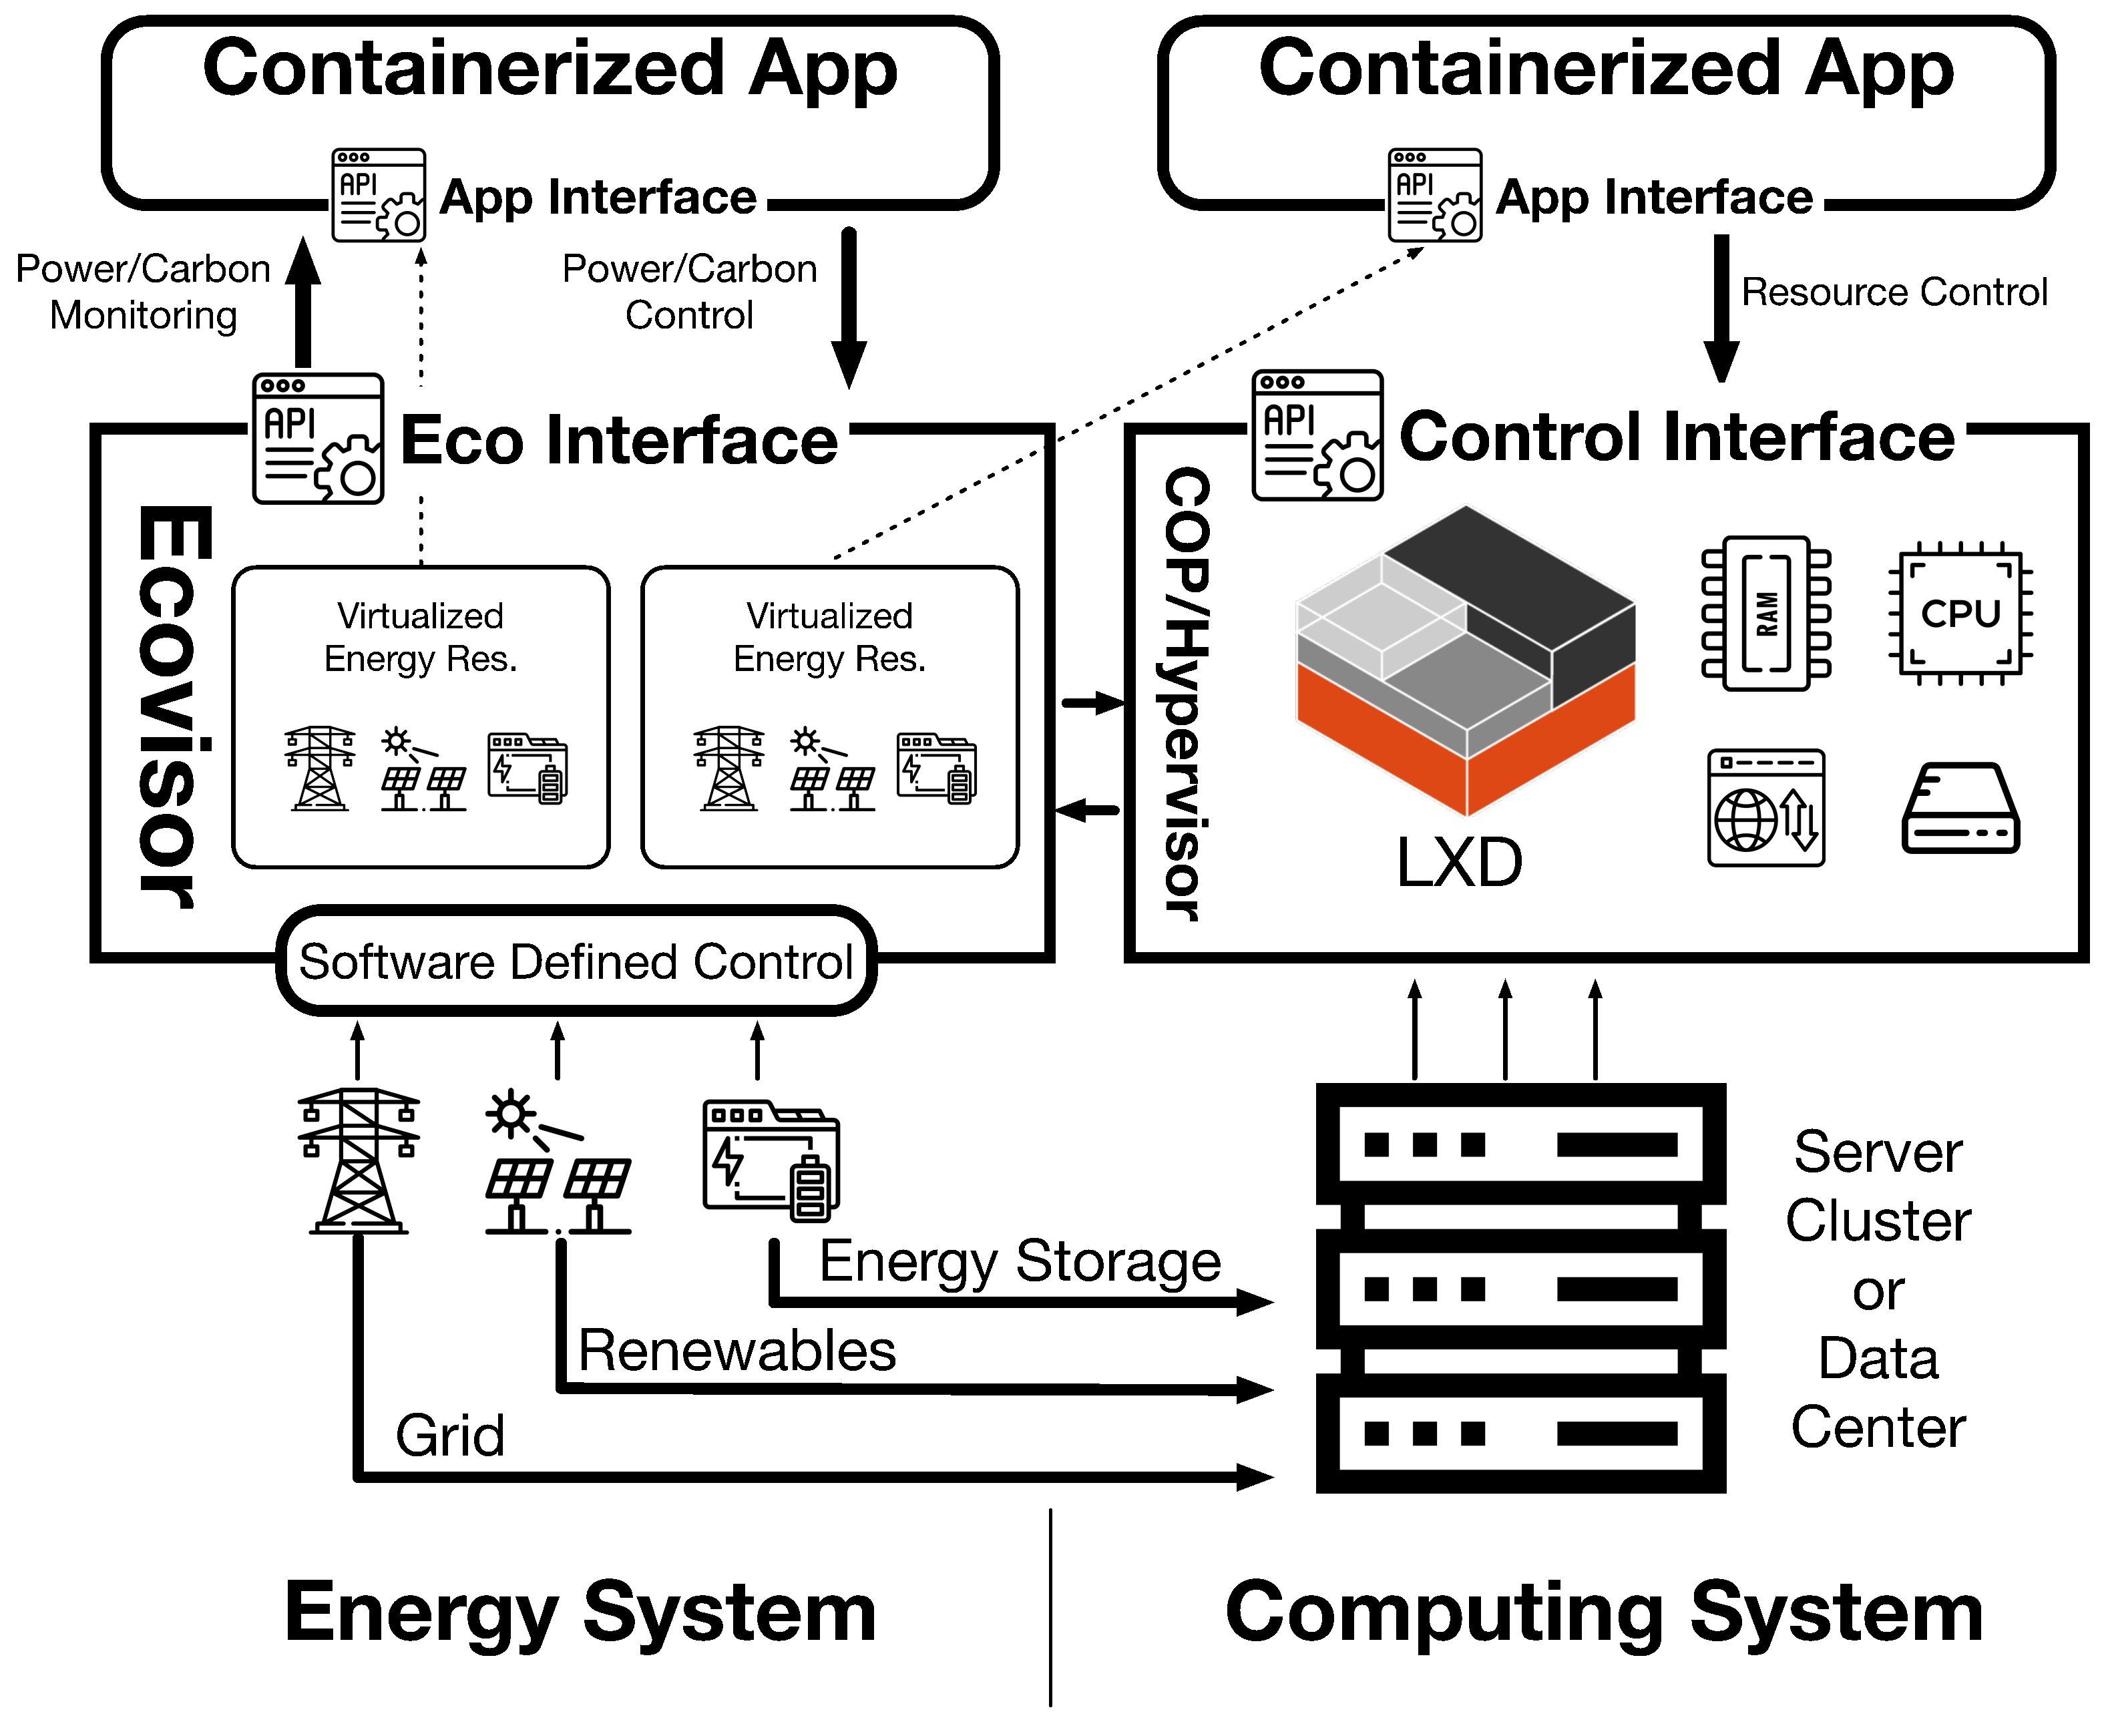
\includegraphics[width=\linewidth]{figures/ecovisor_design}
    \caption{Ecovisor Design (Souza et al.) \cite{souza2023}}
    \label{fig:ecovisor_design}
\end{figure}
